% Options for packages loaded elsewhere
\PassOptionsToPackage{unicode}{hyperref}
\PassOptionsToPackage{hyphens}{url}
\PassOptionsToPackage{dvipsnames,svgnames,x11names}{xcolor}
%
\documentclass[
  letterpaper,
  DIV=11,
  numbers=noendperiod]{scrreprt}

\usepackage{amsmath,amssymb}
\usepackage{iftex}
\ifPDFTeX
  \usepackage[T1]{fontenc}
  \usepackage[utf8]{inputenc}
  \usepackage{textcomp} % provide euro and other symbols
\else % if luatex or xetex
  \usepackage{unicode-math}
  \defaultfontfeatures{Scale=MatchLowercase}
  \defaultfontfeatures[\rmfamily]{Ligatures=TeX,Scale=1}
\fi
\usepackage{lmodern}
\ifPDFTeX\else  
    % xetex/luatex font selection
\fi
% Use upquote if available, for straight quotes in verbatim environments
\IfFileExists{upquote.sty}{\usepackage{upquote}}{}
\IfFileExists{microtype.sty}{% use microtype if available
  \usepackage[]{microtype}
  \UseMicrotypeSet[protrusion]{basicmath} % disable protrusion for tt fonts
}{}
\makeatletter
\@ifundefined{KOMAClassName}{% if non-KOMA class
  \IfFileExists{parskip.sty}{%
    \usepackage{parskip}
  }{% else
    \setlength{\parindent}{0pt}
    \setlength{\parskip}{6pt plus 2pt minus 1pt}}
}{% if KOMA class
  \KOMAoptions{parskip=half}}
\makeatother
\usepackage{xcolor}
\setlength{\emergencystretch}{3em} % prevent overfull lines
\setcounter{secnumdepth}{5}
% Make \paragraph and \subparagraph free-standing
\ifx\paragraph\undefined\else
  \let\oldparagraph\paragraph
  \renewcommand{\paragraph}[1]{\oldparagraph{#1}\mbox{}}
\fi
\ifx\subparagraph\undefined\else
  \let\oldsubparagraph\subparagraph
  \renewcommand{\subparagraph}[1]{\oldsubparagraph{#1}\mbox{}}
\fi

\usepackage{color}
\usepackage{fancyvrb}
\newcommand{\VerbBar}{|}
\newcommand{\VERB}{\Verb[commandchars=\\\{\}]}
\DefineVerbatimEnvironment{Highlighting}{Verbatim}{commandchars=\\\{\}}
% Add ',fontsize=\small' for more characters per line
\usepackage{framed}
\definecolor{shadecolor}{RGB}{241,243,245}
\newenvironment{Shaded}{\begin{snugshade}}{\end{snugshade}}
\newcommand{\AlertTok}[1]{\textcolor[rgb]{0.68,0.00,0.00}{#1}}
\newcommand{\AnnotationTok}[1]{\textcolor[rgb]{0.37,0.37,0.37}{#1}}
\newcommand{\AttributeTok}[1]{\textcolor[rgb]{0.40,0.45,0.13}{#1}}
\newcommand{\BaseNTok}[1]{\textcolor[rgb]{0.68,0.00,0.00}{#1}}
\newcommand{\BuiltInTok}[1]{\textcolor[rgb]{0.00,0.23,0.31}{#1}}
\newcommand{\CharTok}[1]{\textcolor[rgb]{0.13,0.47,0.30}{#1}}
\newcommand{\CommentTok}[1]{\textcolor[rgb]{0.37,0.37,0.37}{#1}}
\newcommand{\CommentVarTok}[1]{\textcolor[rgb]{0.37,0.37,0.37}{\textit{#1}}}
\newcommand{\ConstantTok}[1]{\textcolor[rgb]{0.56,0.35,0.01}{#1}}
\newcommand{\ControlFlowTok}[1]{\textcolor[rgb]{0.00,0.23,0.31}{#1}}
\newcommand{\DataTypeTok}[1]{\textcolor[rgb]{0.68,0.00,0.00}{#1}}
\newcommand{\DecValTok}[1]{\textcolor[rgb]{0.68,0.00,0.00}{#1}}
\newcommand{\DocumentationTok}[1]{\textcolor[rgb]{0.37,0.37,0.37}{\textit{#1}}}
\newcommand{\ErrorTok}[1]{\textcolor[rgb]{0.68,0.00,0.00}{#1}}
\newcommand{\ExtensionTok}[1]{\textcolor[rgb]{0.00,0.23,0.31}{#1}}
\newcommand{\FloatTok}[1]{\textcolor[rgb]{0.68,0.00,0.00}{#1}}
\newcommand{\FunctionTok}[1]{\textcolor[rgb]{0.28,0.35,0.67}{#1}}
\newcommand{\ImportTok}[1]{\textcolor[rgb]{0.00,0.46,0.62}{#1}}
\newcommand{\InformationTok}[1]{\textcolor[rgb]{0.37,0.37,0.37}{#1}}
\newcommand{\KeywordTok}[1]{\textcolor[rgb]{0.00,0.23,0.31}{#1}}
\newcommand{\NormalTok}[1]{\textcolor[rgb]{0.00,0.23,0.31}{#1}}
\newcommand{\OperatorTok}[1]{\textcolor[rgb]{0.37,0.37,0.37}{#1}}
\newcommand{\OtherTok}[1]{\textcolor[rgb]{0.00,0.23,0.31}{#1}}
\newcommand{\PreprocessorTok}[1]{\textcolor[rgb]{0.68,0.00,0.00}{#1}}
\newcommand{\RegionMarkerTok}[1]{\textcolor[rgb]{0.00,0.23,0.31}{#1}}
\newcommand{\SpecialCharTok}[1]{\textcolor[rgb]{0.37,0.37,0.37}{#1}}
\newcommand{\SpecialStringTok}[1]{\textcolor[rgb]{0.13,0.47,0.30}{#1}}
\newcommand{\StringTok}[1]{\textcolor[rgb]{0.13,0.47,0.30}{#1}}
\newcommand{\VariableTok}[1]{\textcolor[rgb]{0.07,0.07,0.07}{#1}}
\newcommand{\VerbatimStringTok}[1]{\textcolor[rgb]{0.13,0.47,0.30}{#1}}
\newcommand{\WarningTok}[1]{\textcolor[rgb]{0.37,0.37,0.37}{\textit{#1}}}

\providecommand{\tightlist}{%
  \setlength{\itemsep}{0pt}\setlength{\parskip}{0pt}}\usepackage{longtable,booktabs,array}
\usepackage{calc} % for calculating minipage widths
% Correct order of tables after \paragraph or \subparagraph
\usepackage{etoolbox}
\makeatletter
\patchcmd\longtable{\par}{\if@noskipsec\mbox{}\fi\par}{}{}
\makeatother
% Allow footnotes in longtable head/foot
\IfFileExists{footnotehyper.sty}{\usepackage{footnotehyper}}{\usepackage{footnote}}
\makesavenoteenv{longtable}
\usepackage{graphicx}
\makeatletter
\def\maxwidth{\ifdim\Gin@nat@width>\linewidth\linewidth\else\Gin@nat@width\fi}
\def\maxheight{\ifdim\Gin@nat@height>\textheight\textheight\else\Gin@nat@height\fi}
\makeatother
% Scale images if necessary, so that they will not overflow the page
% margins by default, and it is still possible to overwrite the defaults
% using explicit options in \includegraphics[width, height, ...]{}
\setkeys{Gin}{width=\maxwidth,height=\maxheight,keepaspectratio}
% Set default figure placement to htbp
\makeatletter
\def\fps@figure{htbp}
\makeatother
% definitions for citeproc citations
\NewDocumentCommand\citeproctext{}{}
\NewDocumentCommand\citeproc{mm}{%
  \begingroup\def\citeproctext{#2}\cite{#1}\endgroup}
\makeatletter
 % allow citations to break across lines
 \let\@cite@ofmt\@firstofone
 % avoid brackets around text for \cite:
 \def\@biblabel#1{}
 \def\@cite#1#2{{#1\if@tempswa , #2\fi}}
\makeatother
\newlength{\cslhangindent}
\setlength{\cslhangindent}{1.5em}
\newlength{\csllabelwidth}
\setlength{\csllabelwidth}{3em}
\newenvironment{CSLReferences}[2] % #1 hanging-indent, #2 entry-spacing
 {\begin{list}{}{%
  \setlength{\itemindent}{0pt}
  \setlength{\leftmargin}{0pt}
  \setlength{\parsep}{0pt}
  % turn on hanging indent if param 1 is 1
  \ifodd #1
   \setlength{\leftmargin}{\cslhangindent}
   \setlength{\itemindent}{-1\cslhangindent}
  \fi
  % set entry spacing
  \setlength{\itemsep}{#2\baselineskip}}}
 {\end{list}}
\usepackage{calc}
\newcommand{\CSLBlock}[1]{\hfill\break\parbox[t]{\linewidth}{\strut\ignorespaces#1\strut}}
\newcommand{\CSLLeftMargin}[1]{\parbox[t]{\csllabelwidth}{\strut#1\strut}}
\newcommand{\CSLRightInline}[1]{\parbox[t]{\linewidth - \csllabelwidth}{\strut#1\strut}}
\newcommand{\CSLIndent}[1]{\hspace{\cslhangindent}#1}

\KOMAoption{captions}{tableheading}
\makeatletter
\@ifpackageloaded{tcolorbox}{}{\usepackage[skins,breakable]{tcolorbox}}
\@ifpackageloaded{fontawesome5}{}{\usepackage{fontawesome5}}
\definecolor{quarto-callout-color}{HTML}{909090}
\definecolor{quarto-callout-note-color}{HTML}{0758E5}
\definecolor{quarto-callout-important-color}{HTML}{CC1914}
\definecolor{quarto-callout-warning-color}{HTML}{EB9113}
\definecolor{quarto-callout-tip-color}{HTML}{00A047}
\definecolor{quarto-callout-caution-color}{HTML}{FC5300}
\definecolor{quarto-callout-color-frame}{HTML}{acacac}
\definecolor{quarto-callout-note-color-frame}{HTML}{4582ec}
\definecolor{quarto-callout-important-color-frame}{HTML}{d9534f}
\definecolor{quarto-callout-warning-color-frame}{HTML}{f0ad4e}
\definecolor{quarto-callout-tip-color-frame}{HTML}{02b875}
\definecolor{quarto-callout-caution-color-frame}{HTML}{fd7e14}
\makeatother
\makeatletter
\@ifpackageloaded{bookmark}{}{\usepackage{bookmark}}
\makeatother
\makeatletter
\@ifpackageloaded{caption}{}{\usepackage{caption}}
\AtBeginDocument{%
\ifdefined\contentsname
  \renewcommand*\contentsname{Table of contents}
\else
  \newcommand\contentsname{Table of contents}
\fi
\ifdefined\listfigurename
  \renewcommand*\listfigurename{List of Figures}
\else
  \newcommand\listfigurename{List of Figures}
\fi
\ifdefined\listtablename
  \renewcommand*\listtablename{List of Tables}
\else
  \newcommand\listtablename{List of Tables}
\fi
\ifdefined\figurename
  \renewcommand*\figurename{Figure}
\else
  \newcommand\figurename{Figure}
\fi
\ifdefined\tablename
  \renewcommand*\tablename{Table}
\else
  \newcommand\tablename{Table}
\fi
}
\@ifpackageloaded{float}{}{\usepackage{float}}
\floatstyle{ruled}
\@ifundefined{c@chapter}{\newfloat{codelisting}{h}{lop}}{\newfloat{codelisting}{h}{lop}[chapter]}
\floatname{codelisting}{Listing}
\newcommand*\listoflistings{\listof{codelisting}{List of Listings}}
\makeatother
\makeatletter
\makeatother
\makeatletter
\@ifpackageloaded{caption}{}{\usepackage{caption}}
\@ifpackageloaded{subcaption}{}{\usepackage{subcaption}}
\makeatother
\makeatletter
\@ifpackageloaded{tikz}{}{\usepackage{tikz}}
\makeatother
        \newcommand*\circled[1]{\tikz[baseline=(char.base)]{
          \node[shape=circle,draw,inner sep=1pt] (char) {{\scriptsize#1}};}}  
                  
\ifLuaTeX
  \usepackage{selnolig}  % disable illegal ligatures
\fi
\usepackage{bookmark}

\IfFileExists{xurl.sty}{\usepackage{xurl}}{} % add URL line breaks if available
\urlstyle{same} % disable monospaced font for URLs
\hypersetup{
  pdftitle={Getting Started},
  pdfauthor={David G. Oppenheimer},
  colorlinks=true,
  linkcolor={blue},
  filecolor={Maroon},
  citecolor={Blue},
  urlcolor={Blue},
  pdfcreator={LaTeX via pandoc}}

\title{Getting Started}
\author{David G. Oppenheimer}
\date{2024-10-02}

\begin{document}
\maketitle

\renewcommand*\contentsname{Table of contents}
{
\hypersetup{linkcolor=}
\setcounter{tocdepth}{2}
\tableofcontents
}
\bookmarksetup{startatroot}

\chapter*{Preface}\label{preface}
\addcontentsline{toc}{chapter}{Preface}

\markboth{Preface}{Preface}

This is a Quarto book.

To learn more about Quarto books visit
\url{https://quarto.org/docs/books}.

\begin{Shaded}
\begin{Highlighting}[]
\DecValTok{1} \SpecialCharTok{+} \DecValTok{1}
\end{Highlighting}
\end{Shaded}

\begin{verbatim}
[1] 2
\end{verbatim}

\bookmarksetup{startatroot}

\chapter{Introduction}\label{introduction}

This is a book created from markdown and executable code.

See Knuth (1984) for additional discussion of literate programming.

\begin{Shaded}
\begin{Highlighting}[]
\DecValTok{1} \SpecialCharTok{+} \DecValTok{1}
\end{Highlighting}
\end{Shaded}

\begin{verbatim}
[1] 2
\end{verbatim}

\bookmarksetup{startatroot}

\chapter{Summary}\label{summary}

In summary, this book has no content whatsoever.

\begin{Shaded}
\begin{Highlighting}[]
\DecValTok{1} \SpecialCharTok{+} \DecValTok{1}
\end{Highlighting}
\end{Shaded}

\begin{verbatim}
[1] 2
\end{verbatim}

\bookmarksetup{startatroot}

\chapter{Software Needed}\label{sec-software-needed}

\section{R and RStudio}\label{r-and-rstudio}

Go to \href{https://posit.co/download/rstudio-desktop/}{RStudio Desktop
download page} to download the R and RStudio Desktop installers.

\begin{tcolorbox}[enhanced jigsaw, colback=white, breakable, titlerule=0mm, leftrule=.75mm, opacitybacktitle=0.6, bottomtitle=1mm, rightrule=.15mm, coltitle=black, arc=.35mm, bottomrule=.15mm, toprule=.15mm, title=\textcolor{quarto-callout-note-color}{\faInfo}\hspace{0.5em}{Note}, left=2mm, opacityback=0, colbacktitle=quarto-callout-note-color!10!white, colframe=quarto-callout-note-color-frame, toptitle=1mm]

You need to install R first, then RStudio.

\end{tcolorbox}

The R link will take you to the \href{https://cran.rstudio.com/}{The
Comprehensive R Archive Network} where you can download an R installer
for your operating system.

The RStudio link will download the apropriate installer for your
operating system.

Download and launch the installers and follow the installation
instructions.

\section{Git and a GitHub Account}\label{git-and-a-github-account}

\href{https://github.com/carpentries-incubator/reproducible-publications-quarto/blob/main/setup.md}{Git
and GitHub}

\begin{tcolorbox}[enhanced jigsaw, colback=white, breakable, titlerule=0mm, leftrule=.75mm, opacitybacktitle=0.6, bottomtitle=1mm, rightrule=.15mm, coltitle=black, arc=.35mm, bottomrule=.15mm, toprule=.15mm, title=\textcolor{quarto-callout-tip-color}{\faLightbulb}\hspace{0.5em}{Tip}, left=2mm, opacityback=0, colbacktitle=quarto-callout-tip-color!10!white, colframe=quarto-callout-tip-color-frame, toptitle=1mm]

We will use \texttt{git} within RStudio. On macOS, RStudio with echo the
mac terminal. I am using \href{https://ohmyz.sh/}{Oh My Zsh} as my
\texttt{zsh} framework, and \href{https://iterm2.com/}{iTerm2} as my
terminal emulator rather than the macOS default terminal application. I
also have the latest \texttt{git} version installed through
\href{https://brew.sh/}{Homebrew}.

This means that I need to adjust the settings in RStudio to use my
\texttt{zsh} environment. Go to \emph{Tools} → \emph{Global Options} →
\emph{Terminal} and choose \texttt{Zsh} from the drop-down menu for the
\emph{New terminals open with} option.

\end{tcolorbox}

\section{VS Code}\label{vs-code}

Download and launch the installer and follow the instructions.

\href{https://code.visualstudio.com/}{Visual Studio Code}

\section{Zotero}\label{zotero}

\subsection{Zotero Desktop}\label{zotero-desktop}

Zotero is available for macOS, Windows, Linux, and iOS.

Download Zotero from the \href{https://www.zotero.org/}{Zotero website}.

Installation is straightforward, but
\href{Installation\%20Instructions}{installation instructions} are
available if needed.

\subsection{Zotero Connector}\label{zotero-connector}

Also install the
\href{https://chromewebstore.google.com/detail/zotero-connector/ekhagklcjbdpajgpjgmbionohlpdbjgc?pli=1}{Zotero
Connector} for the Chrome web browser for easy importing of items into
your Zotero library.

\subsection{Better BibTeX for Zotero}\label{better-bibtex-for-zotero}

To easily cite references in your Quarto documents in RStudio, install
the \href{https://retorque.re/zotero-better-bibtex/}{Better BibTeX
plugin}.

\subsection{Zotero 7 Beta}\label{zotero-7-beta}

There is a \href{https://www.zotero.org/support/beta_builds}{beta
release for Zotero 7}. This has (I believe) a nicer interface, and new
features. See the
\href{https://forums.zotero.org/discussion/105094/announcing-the-zotero-7-beta}{Zotero
7 beta announcement} for more information.

\section{ChimeraX}\label{chimerax}

\begin{enumerate}
\def\labelenumi{\arabic{enumi}.}
\tightlist
\item
  Go to the
  \href{https://www.cgl.ucsf.edu/chimerax/download.html}{ChimeraX
  download page}.
\item
  Download the installer appropriate for your operating system.
\item
  Accept the license agreement.
\item
  Follow the instructions for your operating system. For example, on
  macOS (M2 chip):
\item
  Open the disk image.
\item
  Drag the ChimeraX application to your Applications folder.
\end{enumerate}

\subsection{ISOLDE plugin for
ChimeraX}\label{isolde-plugin-for-chimerax}

Install the ISOLDE plugin using the ChimeraX Toolshed as instructed on
the \href{https://tristanic.github.io/isolde/download/index.html}{ISOLDE
installation web page}.

\begin{enumerate}
\def\labelenumi{\arabic{enumi}.}
\tightlist
\item
  Open ChimeraX.
\item
  In the ChimeraX menu, go to \emph{Tools} → \emph{More Tools}.
\item
  The ChimeraX Toolshed will open in a new window.
\end{enumerate}

\begin{figure}

\begin{minipage}{0.50\linewidth}

\centering{

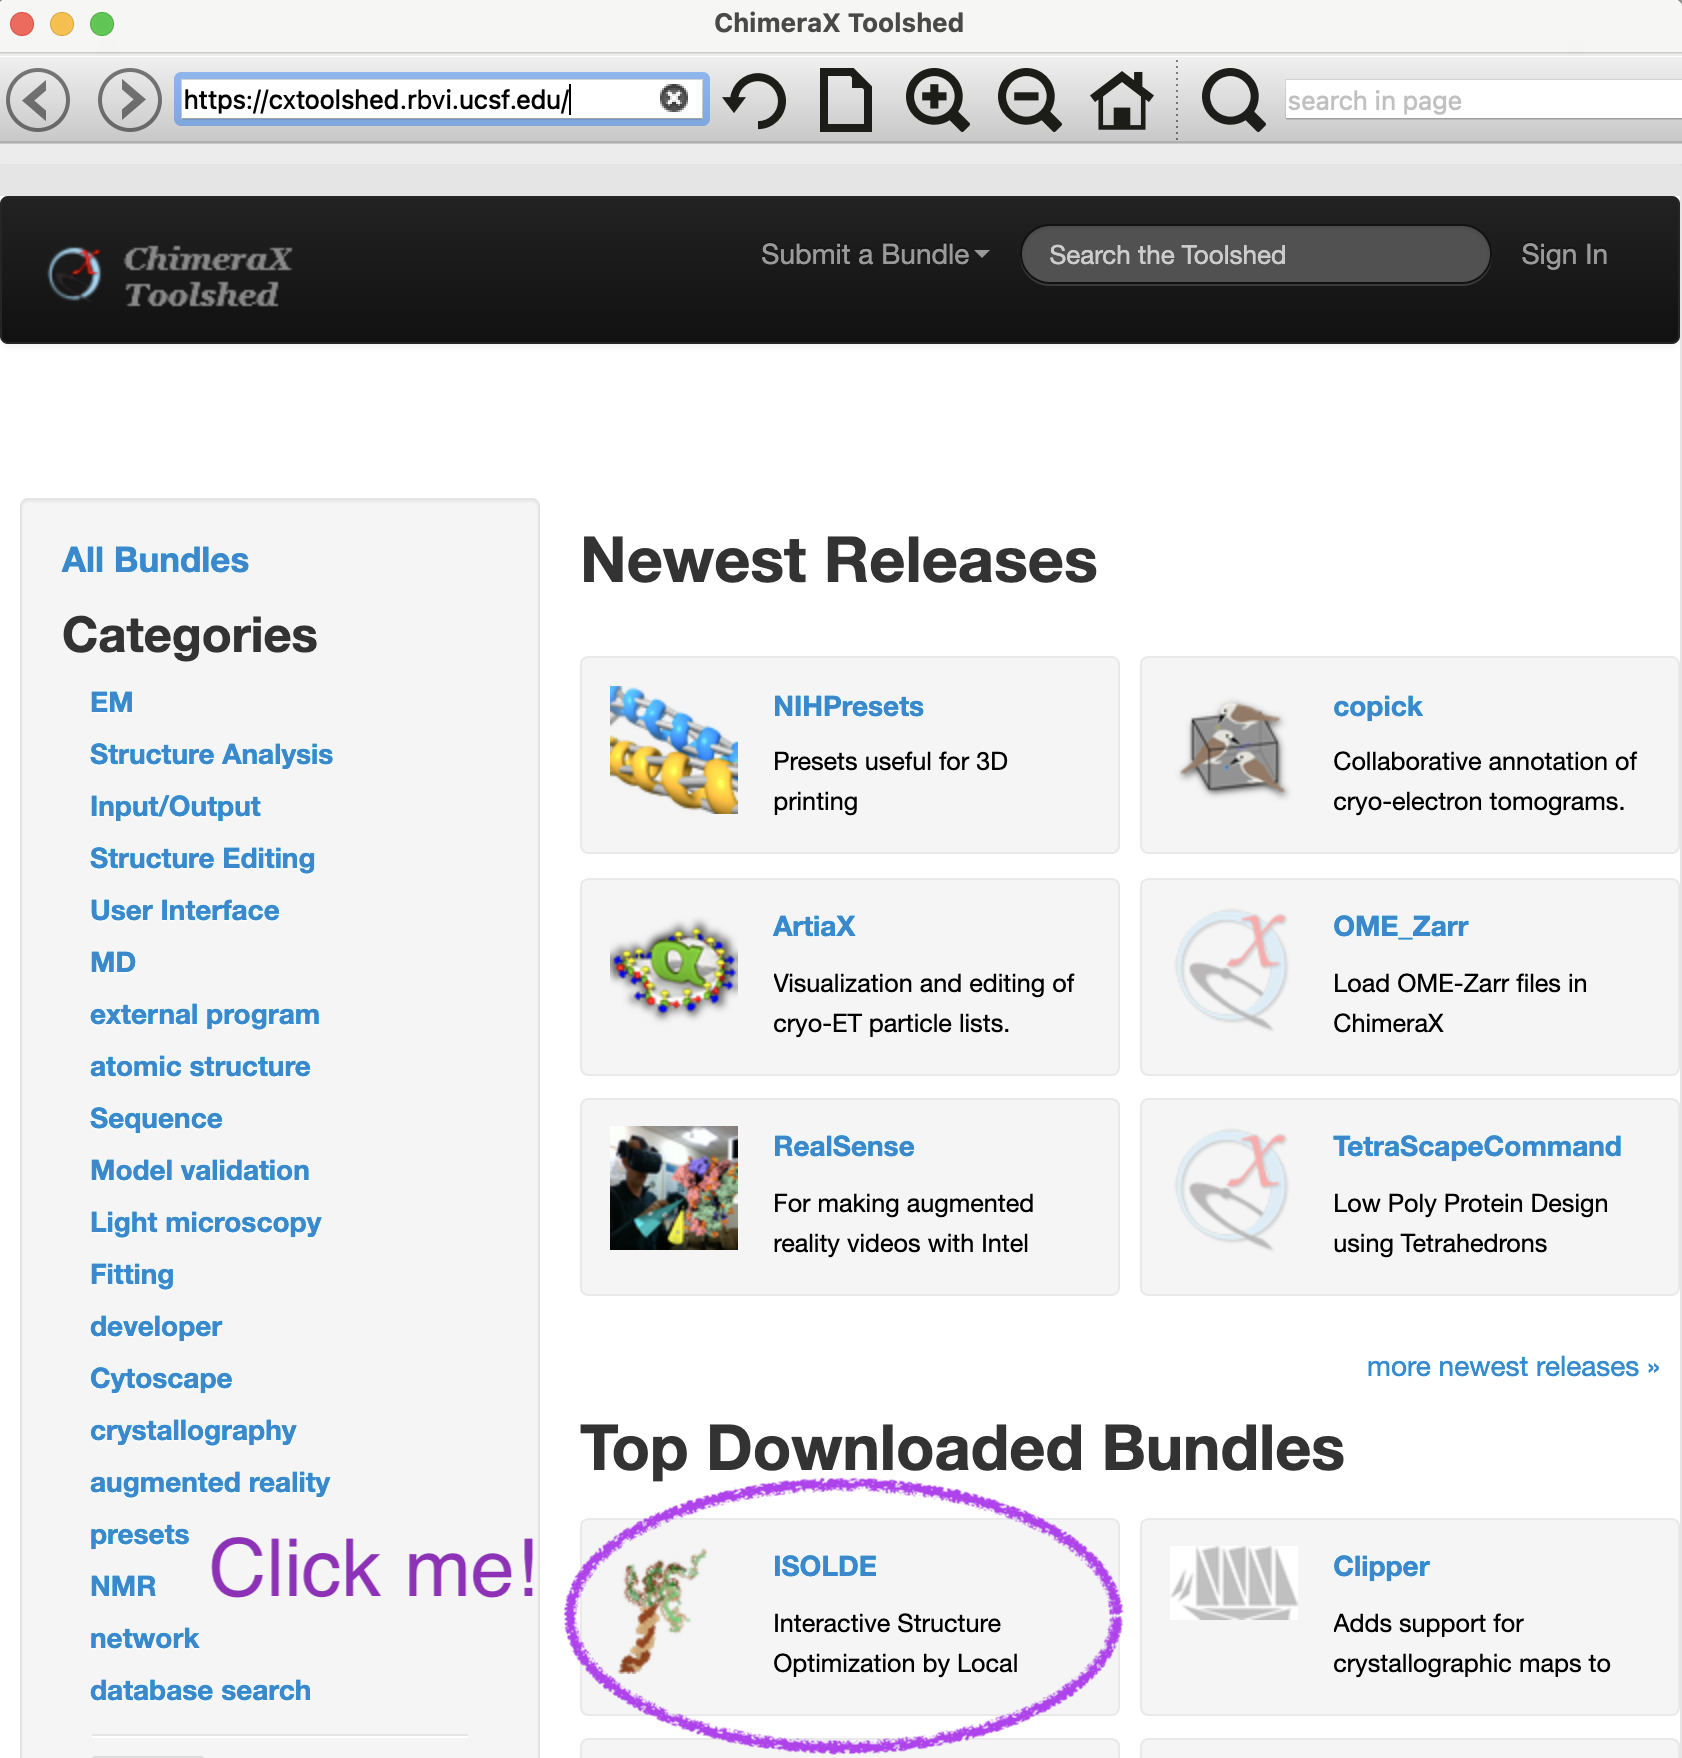
\includegraphics{../assets/chimerax-toolshed.png}

}

\subcaption{\label{fig-toolshed}ChimeraX Toolshed}

\end{minipage}%
%
\begin{minipage}{0.50\linewidth}

\centering{

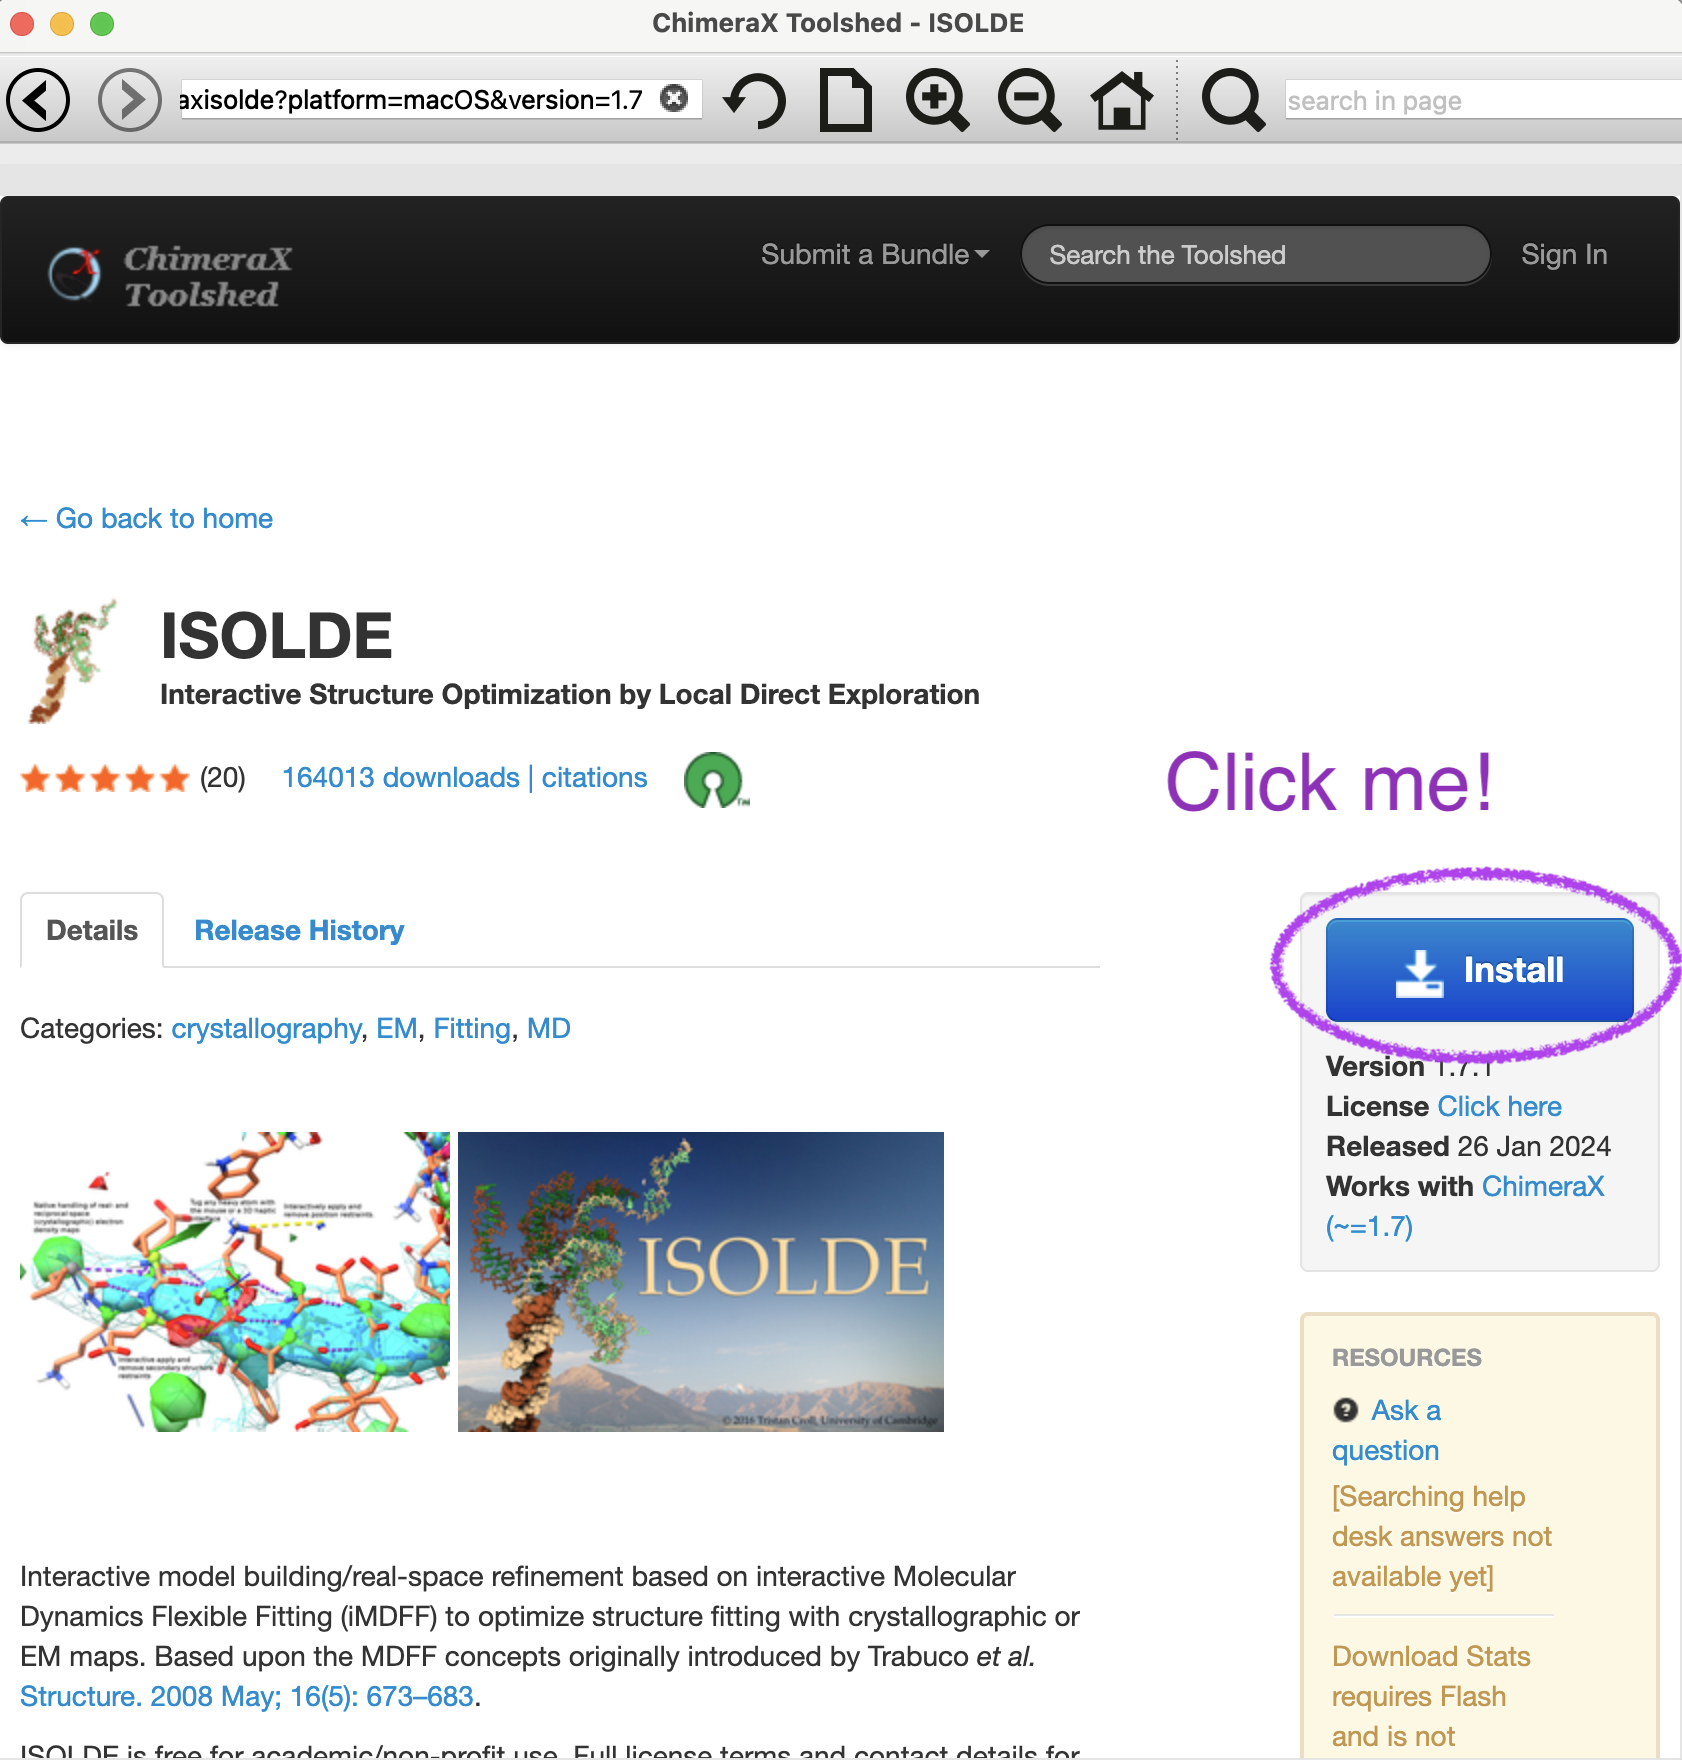
\includegraphics{../assets/isolde-install.png}

}

\subcaption{\label{fig-isolde-install}ISOLDE install button}

\end{minipage}%

\caption{\label{fig-isolde}Installing the ISOLDE plugin in ChimeraX
(\emph{Click image to enlarge})}

\end{figure}%

\begin{enumerate}
\def\labelenumi{\arabic{enumi}.}
\setcounter{enumi}{3}
\tightlist
\item
  Click on the ISOLDE button (Fig. 4.1 a).
\item
  In the resulting window that opens, click on the Install button (Fig.
  4.1 b).
\item
  Wait for the download and installation to complete. A message will
  appear in the ChimeraX log when the installation is done.
\item
  To use ISOLDE, go to \emph{Tools} → \emph{General} → \emph{ISOLDE}.
\end{enumerate}

\section{RealVNC Viewer}\label{realvnc-viewer}

\subsection{RealVNC Viewer}\label{realvnc-viewer-1}

To connect to NMRbox to run GROMACS simulations, you need to install VNC
software. VNC is an abbreviation of Virtual Network Computing, which is
another way to say screen sharing. NMRbox uses
\href{https://www.realvnc.com/en/connect/download/vnc/}{RealVNC Server}
to which we can connect using the client software,
\href{https://www.realvnc.com/en/connect/download/viewer/}{RealVNC
Viewer}.

\href{https://www.realvnc.com/en/connect/download/viewer/}{Download} and
install the software following the onscreen instructions (for macOS,
drag the app to the \emph{Applications} folder).

\subsubsection{Troubleshooting}\label{troubleshooting}

\begin{description}
\item[copy and paste to NMRbox stops working]
In Terminal on NMRbox, type the following: \texttt{vncconfig\ \&} and
hit return. See
\href{https://www.anyviewer.com/how-to/vnc-viewer-copy-paste-2578.html}{How
to fix VNC Viewer copy-paste not working} for additional help.
\end{description}

\section{AmberTools}\label{ambertools}

We need to use the \emph{AmberTools} program, \texttt{tleap}, to
generate the IDP fragments to generate the fragment library. We will
install the \texttt{conda} version of \emph{AmberTools}.

\begin{enumerate}
\def\labelenumi{\arabic{enumi}.}
\tightlist
\item
  Go to the \href{https://ambermd.org/GetAmber.php}{Amber Download
  page}.
\item
  Choose \emph{Option 1: Binary distribution via conda}.
\item
  Type the following into a Terminal:
\end{enumerate}

\begin{codelisting}

\caption{\texttt{Terminal}}

\begin{Shaded}
\begin{Highlighting}[]
\ExtensionTok{conda}\NormalTok{ create }\AttributeTok{{-}{-}name}\NormalTok{ AmberTools23}
\ExtensionTok{conda}\NormalTok{ activate AmberTools23}
\end{Highlighting}
\end{Shaded}

\end{codelisting}

\begin{tcolorbox}[enhanced jigsaw, colback=white, breakable, titlerule=0mm, leftrule=.75mm, opacitybacktitle=0.6, bottomtitle=1mm, rightrule=.15mm, coltitle=black, arc=.35mm, bottomrule=.15mm, toprule=.15mm, title=\textcolor{quarto-callout-note-color}{\faInfo}\hspace{0.5em}{Note}, left=2mm, opacityback=0, colbacktitle=quarto-callout-note-color!10!white, colframe=quarto-callout-note-color-frame, toptitle=1mm]

From the \href{https://ambermd.org/GetAmber.php}{AmberTools installation
page}:

\begin{quote}
Note that you would need to perform the ``conda activate'' step every
time you wish use AmberTools23 in a new terminal
\end{quote}

To deactivate a \texttt{conda} environment, just use

\begin{codelisting}[H]

\caption{\texttt{Terminal}}

\begin{Shaded}
\begin{Highlighting}[]
\ExtensionTok{conda}\NormalTok{ deactivate}
\end{Highlighting}
\end{Shaded}

\end{codelisting}

\end{tcolorbox}

\begin{enumerate}
\def\labelenumi{\arabic{enumi}.}
\setcounter{enumi}{3}
\tightlist
\item
  Next type:
\end{enumerate}

\begin{codelisting}

\caption{\texttt{Terminal}}

\begin{Shaded}
\begin{Highlighting}[]
\ExtensionTok{conda}\NormalTok{ install }\AttributeTok{{-}c}\NormalTok{ conda{-}forge ambertools=23}
\end{Highlighting}
\end{Shaded}

\end{codelisting}

\begin{tcolorbox}[enhanced jigsaw, colback=white, breakable, titlerule=0mm, leftrule=.75mm, opacitybacktitle=0.6, bottomtitle=1mm, rightrule=.15mm, coltitle=black, arc=.35mm, bottomrule=.15mm, toprule=.15mm, title=\textcolor{quarto-callout-note-color}{\faInfo}\hspace{0.5em}{Note}, left=2mm, opacityback=0, colbacktitle=quarto-callout-note-color!10!white, colframe=quarto-callout-note-color-frame, toptitle=1mm]

To keep \emph{AmberTools} up to date, type the following:

\begin{codelisting}[H]

\caption{\texttt{Terminal}}

\begin{Shaded}
\begin{Highlighting}[]
\ExtensionTok{conda}\NormalTok{ update }\AttributeTok{{-}c}\NormalTok{ conda{-}forge ambertools}
\end{Highlighting}
\end{Shaded}

\end{codelisting}

\end{tcolorbox}

\section{Optional Software}\label{optional-software}

\subsection{Anaconda}\label{anaconda}

\subsubsection{Update Homebrew}\label{update-homebrew}

In terminal:

\phantomsection\label{annotated-cell-6}%
\begin{Shaded}
\begin{Highlighting}[]
\BuiltInTok{cd}\NormalTok{ \textasciitilde{}}
\ExtensionTok{brew}\NormalTok{ update }\hspace*{\fill}\NormalTok{\circled{1}}
\ExtensionTok{brew}\NormalTok{ upgrade }\hspace*{\fill}\NormalTok{\circled{2}}
\end{Highlighting}
\end{Shaded}

\begin{description}
\tightlist
\item[\circled{1}]
Update the Homebrew package manager.
\item[\circled{2}]
Upgrade the packages in Homebrew. \emph{Note}: This can take a long time
(hours) depending on how many packages need upgrading.
\end{description}

\subsubsection{Install Anaconda}\label{install-anaconda}

\begin{Shaded}
\begin{Highlighting}[]
\NormalTok{brew install }\SpecialCharTok{{-}{-}}\NormalTok{cask anaconda}
\end{Highlighting}
\end{Shaded}

After installation is complete, add the path to \texttt{.zshrc} and
restart shell.

\begin{Shaded}
\begin{Highlighting}[]
\BuiltInTok{echo} \StringTok{\textquotesingle{}export PATH="/usr/local/Homebrew/anaconda3/bin:$PATH"\textquotesingle{}} \OperatorTok{\textgreater{}\textgreater{}}\NormalTok{ \textasciitilde{}/.zshrc}
\BuiltInTok{source}\NormalTok{ \textasciitilde{}/.zshrc}
\end{Highlighting}
\end{Shaded}

\subsubsection{Activate Anaconda}\label{activate-anaconda}

\phantomsection\label{annotated-cell-9}%
\begin{Shaded}
\begin{Highlighting}[]
\BuiltInTok{source}\NormalTok{ /usr/local/Homebrew/anaconda3/bin/activate }\hspace*{\fill}\NormalTok{\circled{1}}
\ExtensionTok{conda}\NormalTok{ init zsh }\hspace*{\fill}\NormalTok{\circled{2}}
\end{Highlighting}
\end{Shaded}

\begin{description}
\tightlist
\item[\circled{1}]
Use the path to the Homebrew-installed Anaconda.
\item[\circled{2}]
Initialize your preferred shell to work with \texttt{conda.}
\end{description}

Test the installation.

\begin{Shaded}
\begin{Highlighting}[]
\ExtensionTok{conda} \AttributeTok{{-}{-}version}
\ExtensionTok{conda}\NormalTok{ 25.4.0}
\end{Highlighting}
\end{Shaded}

✅ Success!

\subsubsection{\texorpdfstring{Create and activate a \texttt{conda}
Environment for the Plumed Masterclass
Tutuorial}{Create and activate a conda Environment for the Plumed Masterclass Tutuorial}}\label{create-and-activate-a-conda-environment-for-the-plumed-masterclass-tutuorial}

\begin{Shaded}
\begin{Highlighting}[]
\ExtensionTok{conda}\NormalTok{ create }\AttributeTok{{-}{-}name}\NormalTok{ plumed{-}masterclass{-}2022}
\end{Highlighting}
\end{Shaded}

Activate the environment with:

\begin{Shaded}
\begin{Highlighting}[]
\ExtensionTok{conda}\NormalTok{ activate plumed{-}masterclass{-}2022}
\end{Highlighting}
\end{Shaded}

\begin{tcolorbox}[enhanced jigsaw, colback=white, breakable, titlerule=0mm, leftrule=.75mm, opacitybacktitle=0.6, bottomtitle=1mm, rightrule=.15mm, coltitle=black, arc=.35mm, bottomrule=.15mm, toprule=.15mm, title=\textcolor{quarto-callout-note-color}{\faInfo}\hspace{0.5em}{Note}, left=2mm, opacityback=0, colbacktitle=quarto-callout-note-color!10!white, colframe=quarto-callout-note-color-frame, toptitle=1mm]

To deactivate an active environment, use

\begin{Shaded}
\begin{Highlighting}[]
\ExtensionTok{conda}\NormalTok{ deactivate}
\end{Highlighting}
\end{Shaded}

\end{tcolorbox}

\bookmarksetup{startatroot}

\chapter{Scratch Pad}\label{scratch-pad}

Just a place for quick notes

\bookmarksetup{startatroot}

\chapter*{References}\label{references}
\addcontentsline{toc}{chapter}{References}

\markboth{References}{References}

\phantomsection\label{refs}
\begin{CSLReferences}{1}{0}
\bibitem[\citeproctext]{ref-knuth84}
Knuth, Donald E. 1984. {``Literate Programming.''} \emph{Comput. J.} 27
(2): 97--111. \url{https://doi.org/10.1093/comjnl/27.2.97}.

\end{CSLReferences}



\end{document}
